% \graphicspath{{../images/graphs/accuracy/} {../images/graphs/parameters/} {../images/graphs/throughput/}}
\chapter{Evaluation}
\label{chap:eval}

In this chapter we measure \mysketch's throughput and accuracy of estimation. 
Section~\ref{sec:setup} presents the experiment setup and methodology.
Section~\ref{sec:tput} presents throughput measurements and discusses scalability.
Section~\ref{sec:params} experiments with different parameter setting, examining how performance is affected by query freshness. 
Section~\ref{sec:accuracy} presents an accuracy of estimation analysis.
Finally, Section~\ref{sec:compare} compares \mysketch\ to the state-of-the-art. 

%============================================================
\section{Setup and Methodology}
\label{sec:setup}
%============================================================
We implement \mysketch in C++. Our memory management system is based on \acrshort{IBR}~\cite{Haosen_2018_IBR}, an interval-based approach to memory reclamation for concurrent data structures. 
The experiments were run on a NUMA system with four Intel Xeon E5-4650 processors, each with 8 cores, for a total of 32 threads (with hyper-threading disabled).


Each thread was pinned to a NUMA node, and nodes were first filled before overflowing to other NUMA nodes, i.e., $8$ threads use only a single node, while $9$ use two nodes with $8$ threads on one and $1$ on the second. The default memory allocation policy is local allocation, except for \mysketch's shared pointers. Each Gather\&Sort unit is allocated on a different NUMA node and threads update the G\&SBuffers allocated on the node they belong to.
The stream is drawn from a uniform distribution, unless stated otherwise. Each data point is an average of 15 runs, to minimize measurement noise.

 
%============================================================
\section{Throughput Scalability}
\label{sec:tput} 
%============================================================
We measured \mysketch's throughput in three workloads:
(1) update-only, (2) query-only, and (3) mixed update-query. In the update-only workload, we update \mysketch with a stream of 10M elements and measure the time it takes to feed the sketch. For the other two workloads, we pre-fill the sketch with a stream of 10M elements and then execute the workload (10M queries only or queries and 10M updates) and measure performance. Figure~\ref{fig:throughput} shows \mysketch's throughput in those workloads with $k = 4096$ and $b = 16$,

\begin{figure*}[h] %throughput
\centering
    % \hspace{-3em}
    \begin{subfigure}[]{0.49\textwidth}
        \centering
        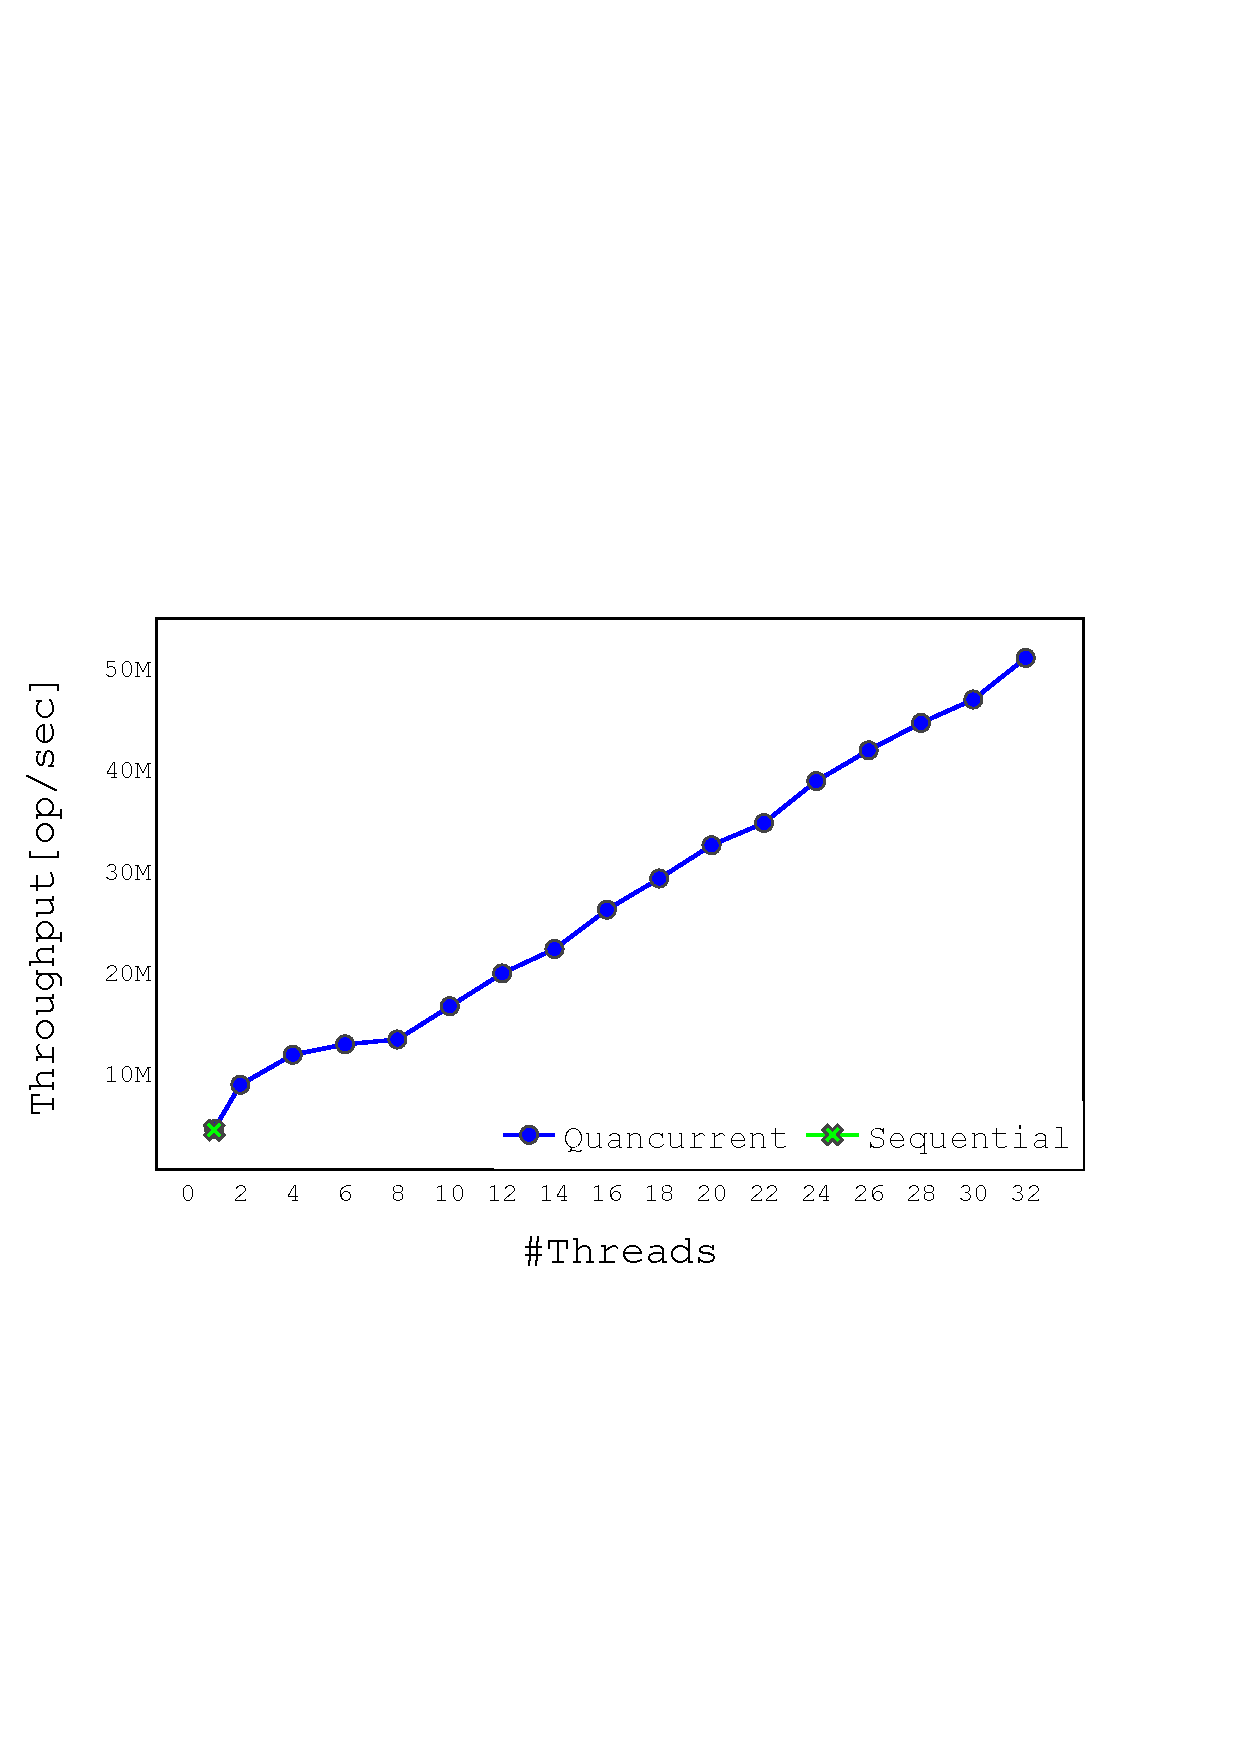
\includegraphics[width=\textwidth,trim={0cm 7cm 1.9cm 10cm},clip] {graphics/graphs/throughput/oracle_Quancurrent_blocking_numa_update_k4096_b16_keys10M_Tup32_runs15_16-08-2022_05-29-07_flat.pdf}
        \caption{Update-only, $10M$ elements.}
        \label{fig:update_only_speedup}
    \end{subfigure}
    % \hspace{-5em}
    \begin{subfigure}[]{0.49\textwidth}
        \centering
        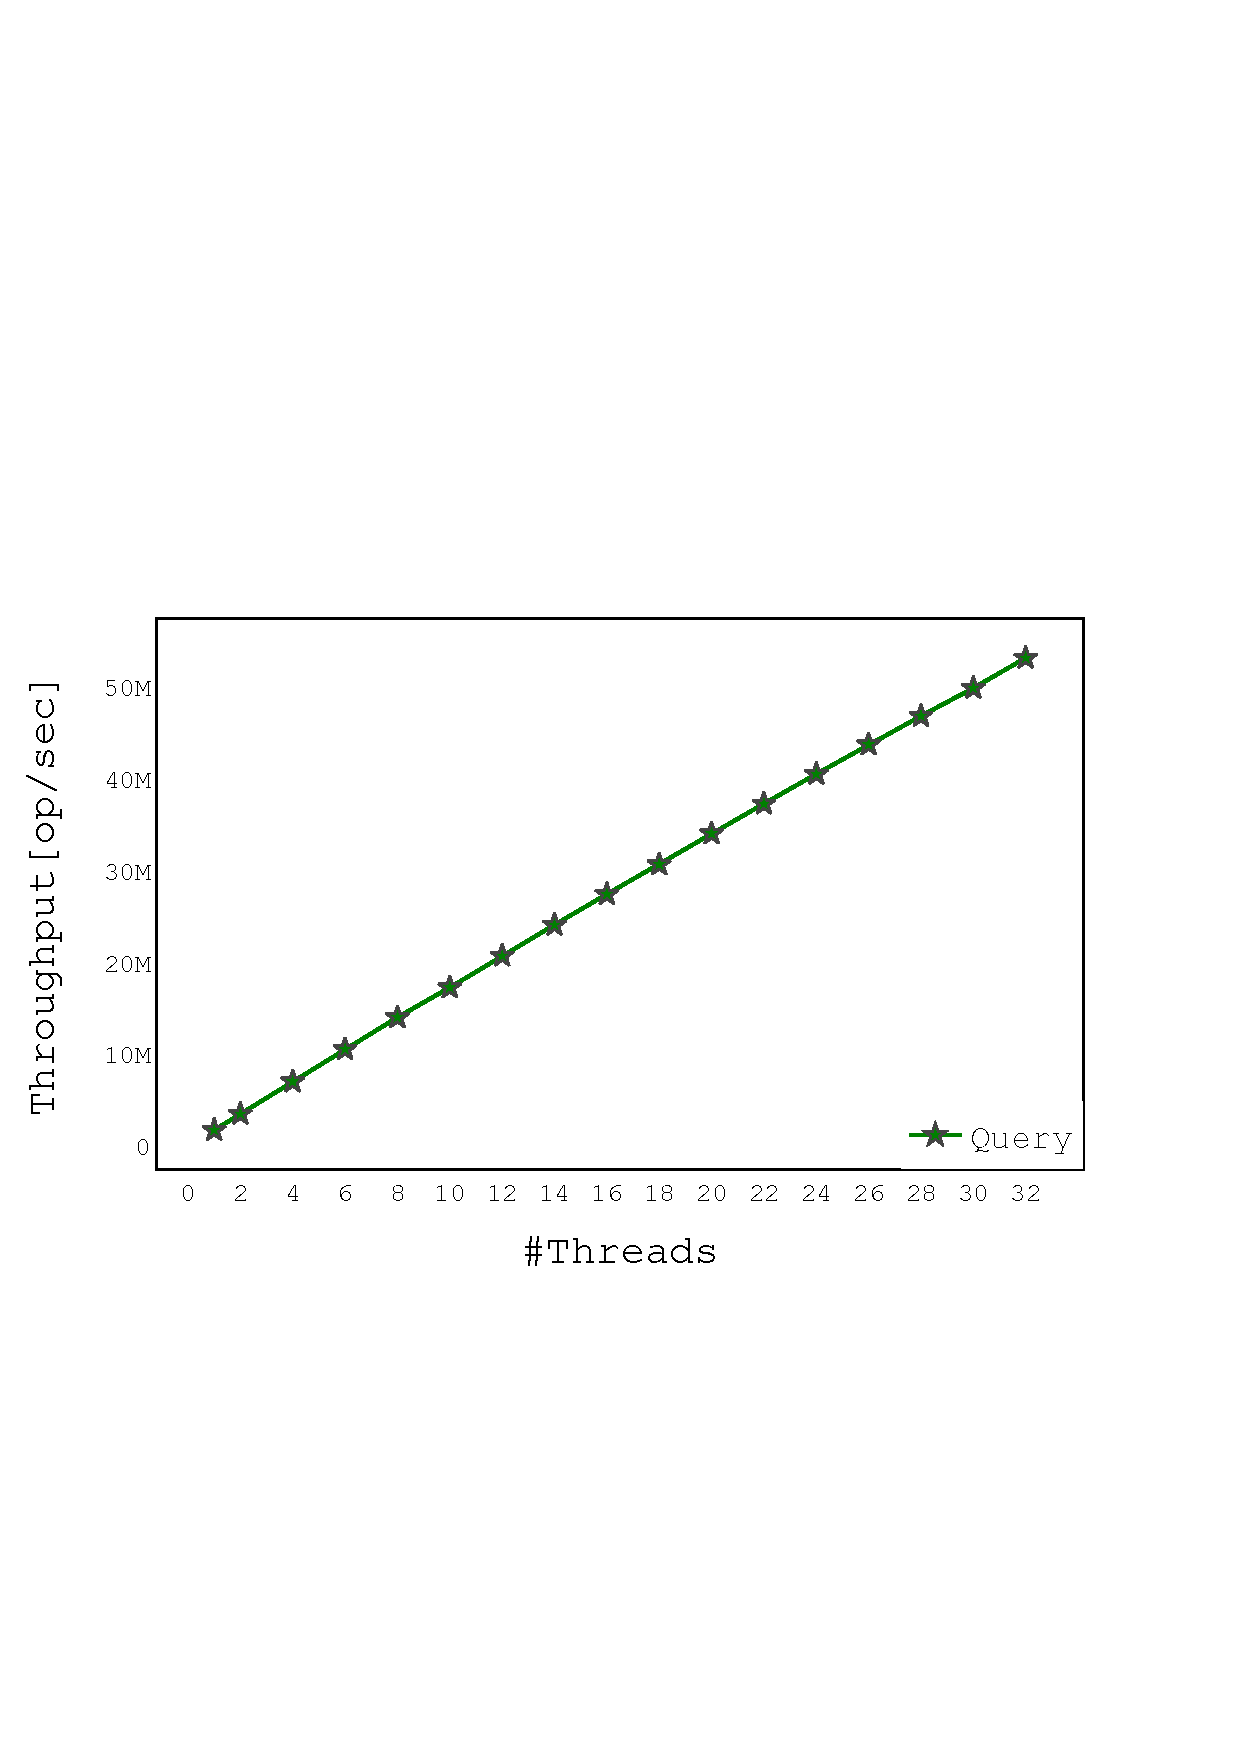
\includegraphics[width=\textwidth,trim={0cm 7cm 1.9cm 9cm},clip] {graphics/graphs/throughput/oracle_Quancurrent_blocking_numa_query_k4096_b16_keys10M_Tup32_runs15_prefill10M_prefillT1_16-08-2022_05-38-28_flat.pdf}
        \caption{Query-only, $10M$ elements prefilled, $10M$ queries.}
        \label{fig:query_only_throughput}
    \end{subfigure}

    \begin{subfigure}[]{\textwidth}
        \centering
        \hspace{5pt}
        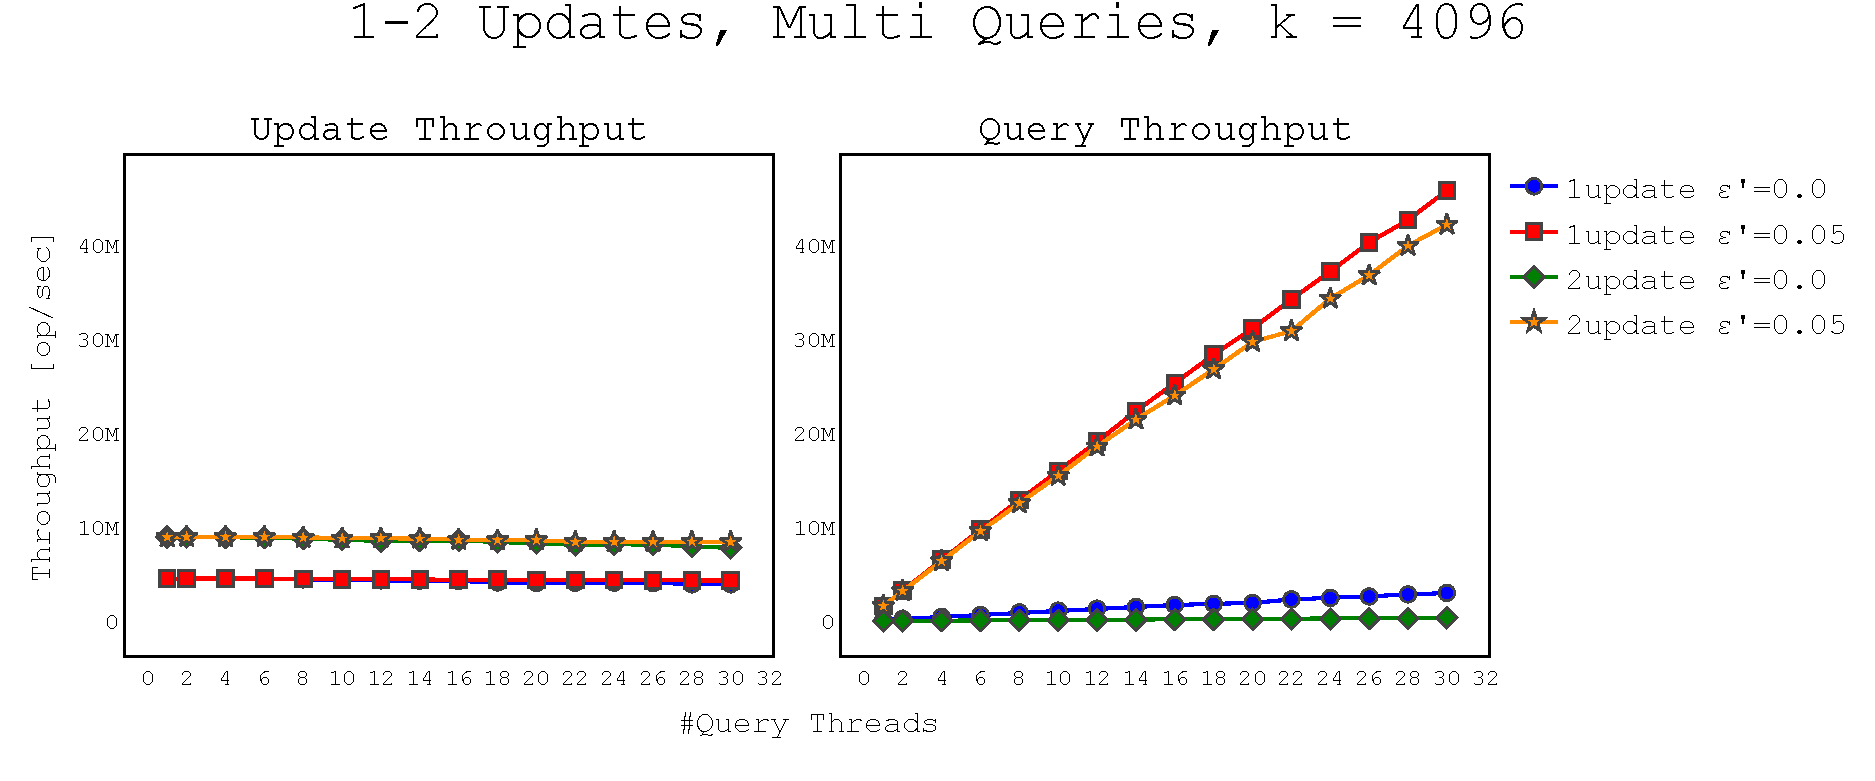
\includegraphics[width=\textwidth,trim={0cm 0cm 0cm 1cm},clip]
        {graphics/graphs/throughput/oracle_Quancurrent_blocking_numa_update_query_k_4096_b16_keys10M_pre10M_preT1_runs15_Tu1-2_Tq2-30_snapshot1_rho_1_0-05_united_16-08-2022_07-09-08.pdf}
        \caption{One or two update threads, up to $32$ query threads, $10M$ elements inserted after a pre-fill of $10M$ elements.}
        \label{fig:mixed_throughput}
    \end{subfigure}
    \caption{\mysketch's throughput, $k=4096$, $b=16$.}
    \label{fig:throughput}
\end{figure*}


As shown in Figure \ref{fig:update_only_speedup}, \mysketch's performance in the update-only workload with a single thread is similar to the sequential algorithm and with more threads it scales linearly, reaching $12x$ the sequential throughput with 32 threads. 
%Recall that the bottleneck of threads on the same NUMA node is sorting the buffer of size $2k$. As described in Section~\ref{Section: concurrent_algorithm}, the first two stages of \mysketch's update operation include filling and sorting threads local buffers and sorting the two G\&SBuffers. Note that the fill can be done concurrently, but the sort is sequential. The first $8$ threads running on the first NUMA node reach a peak and the empirical results match the theoretical expectations. For $N>8$, the throughput increases with the number of threads as adding NUMA nodes increases concurrency.
We observe that the speedup is faster with fewer threads, we believe this is because once there are more than $8$ threads, the shared object is accessed from multiple NUMA nodes.
%, thus the throughput above $8$ threads doesn't scale in the same manner as with the first $8$ threads. 


Figure~\ref{fig:query_only_throughput} shows that, as expected, the throughput of the query-only workload scales linearly with the number of query threads, reaching $30x$ the sequential throughput with 32 threads.


In the mixed workload, the parameter $\rho$ is significant for performance - when $\rho = 1$ ($\epsilon'=0$, no caching), a snapshot it reproduced on every query.
% We compare performance with $\rho = 0$ and $\rho = 0.05$.
Figure~\ref{fig:mixed_throughput} presents the update throughput (left) and query throughput (right) in the presence of $1$ or $2$ update threads, with staleness thresholds of $\rho=1 (\epsilon'=0)$ and $\rho=1.05 (\epsilon'=0.05)$. We see that the caching mechanism ($\rho > 1$) is indeed crucial for performance. As expected, increasing the staleness threshold allows queries to use their local (possibly stale) snapshot, servicing queries faster and greatly increasing the query throughout. Furthermore, more update threads decrease the query throughput, as the update threads interfere with the query snapshot. 
Finally, increasing the number of query threads decreases the update throughput, as query threads interfere with update threads, presumably due to cache invalidations of the shared state.


%============================================================
\section{Parameter Exploration}
\label{sec:params} 
%============================================================
We now experiment with different parameter settings with up to $32$ threads. 
In  Figure~\ref{fig: throughput_update_compare_k} we vary $k$ from $256$ to $4096$, in update-only scenario with $b = 16$ and up to $32$ update threads.
We see that the scalability trends are similar, and that \mysketch's throughput increases with $k$, peaking at $k = 2048$, after which increasing $k$ has little effect.
This illustrates the tradeoff between the sketch size (memory footprint) to  throughput and accuracy. 


Figure~\ref{fig: throughput_update_compare_b} experiments with different local buffer sizes, from $1$ to $64$, in update-only scenario with $k = 4096$ and up to $32$ update threads. Not surprisingly, the throughput increases as the local buffer grows as this enables more concurrency. 
%As Figure~\ref{fig: accuracy_stderr} shows, this does not have a large impact on steady-state accuracy.


In Figure~\ref{fig: update_query_compare_rho} we vary $\rho$, in a mixed update-query workload with $8$ update threads, $24$ query threads, $k = 1024$, and $b = 16$, exploring another aspect of query freshness versus performance. As expected, increasing  $\rho$ has a positive impact on query throughput, as the cached snapshot can be queried more often.  Figure~\ref{fig: update_query_compare_rho} also shows the miss rate, which is the percentage of queries that need to re-construct the snapshot.


\begin{figure*}[htp!]
    \centering
    \begin{subfigure}{\textwidth}
    \centering
    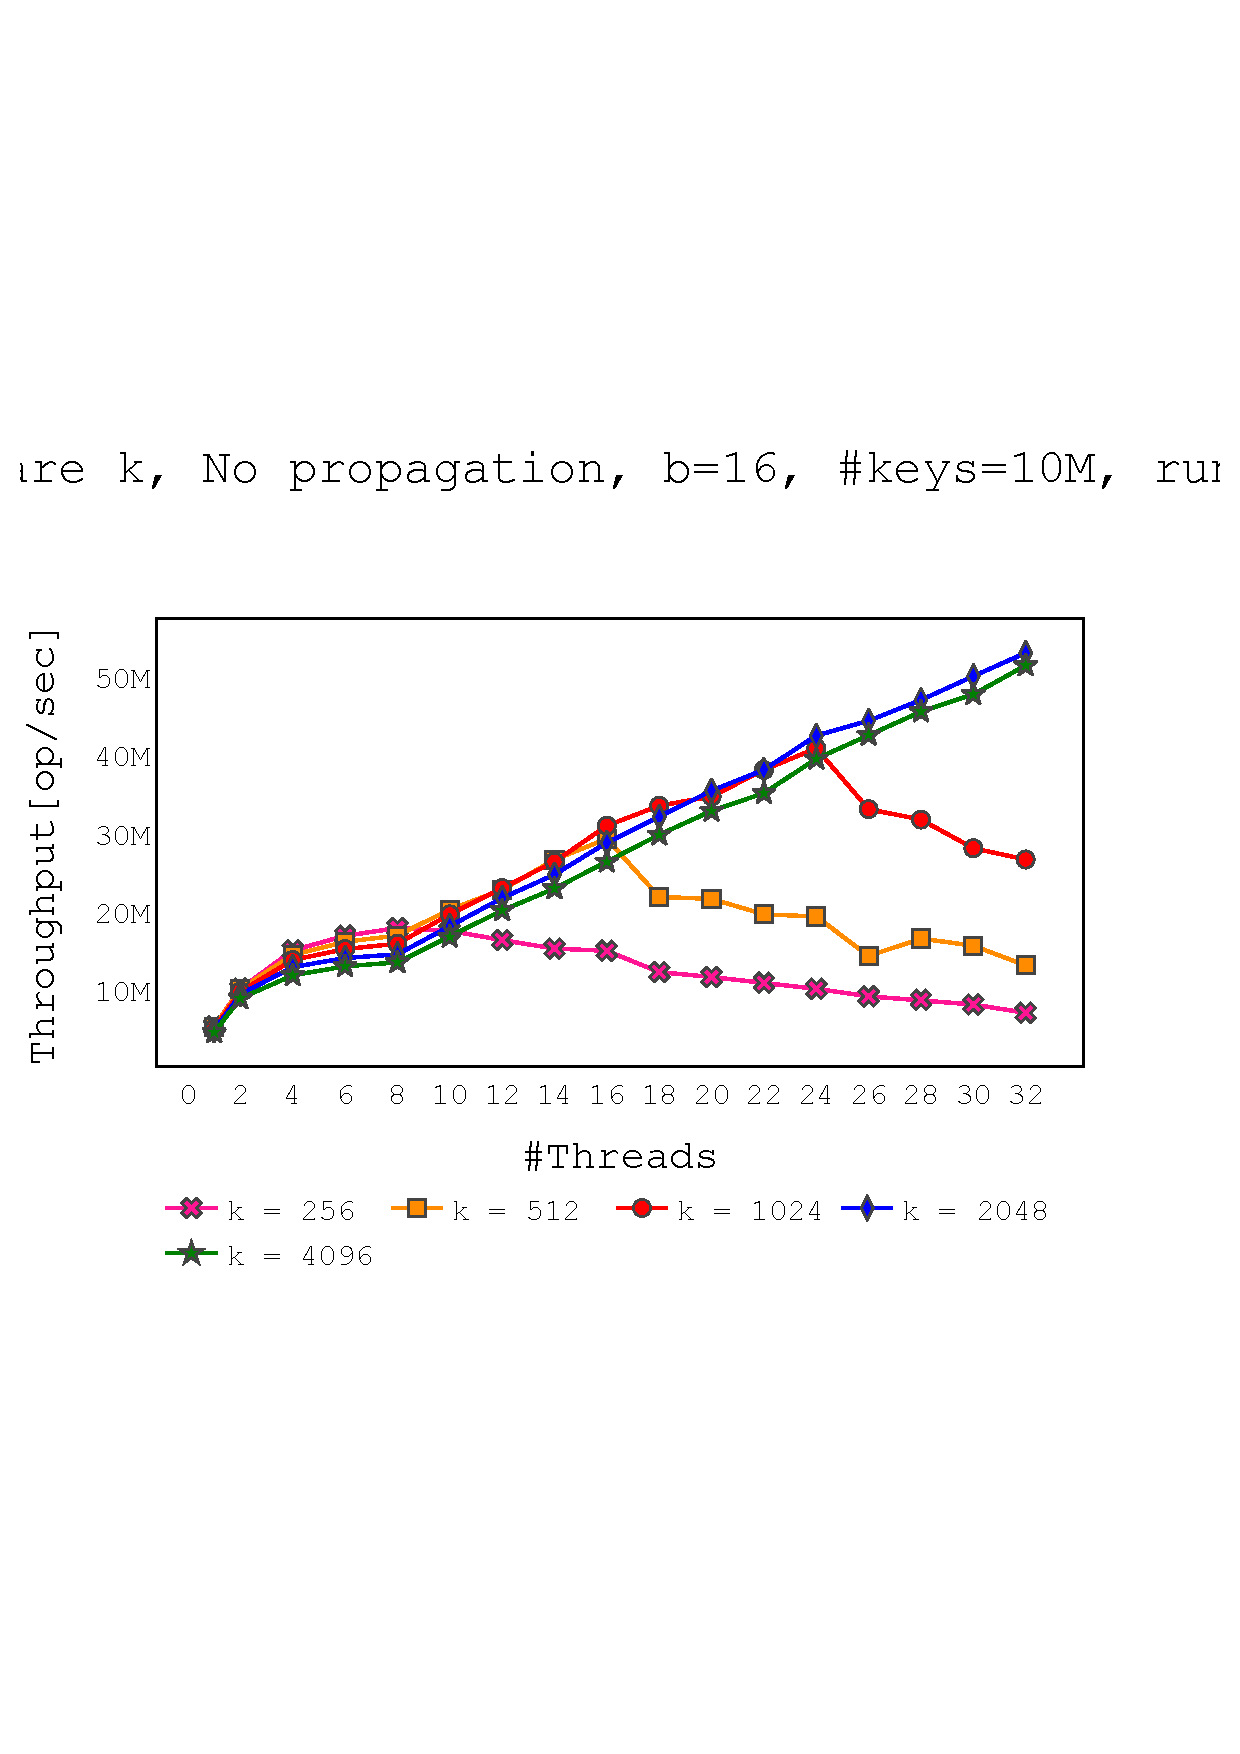
\includegraphics[width=0.7\textwidth,trim={0cm 7cm 1cm 10cm},clip]{graphics/graphs/parameters/oracle_Quancurrent_blocking_numa_compare_k_b16_keys10M_Tup32_runs15_04-07-2022_12-26-29_flat.pdf}
    \caption{Update-only, \#keys = $10M$, $b=16$.}
    \label{fig: throughput_update_compare_k}
    \end{subfigure}
\vfill
    \begin{subfigure}{\textwidth}
    \centering
    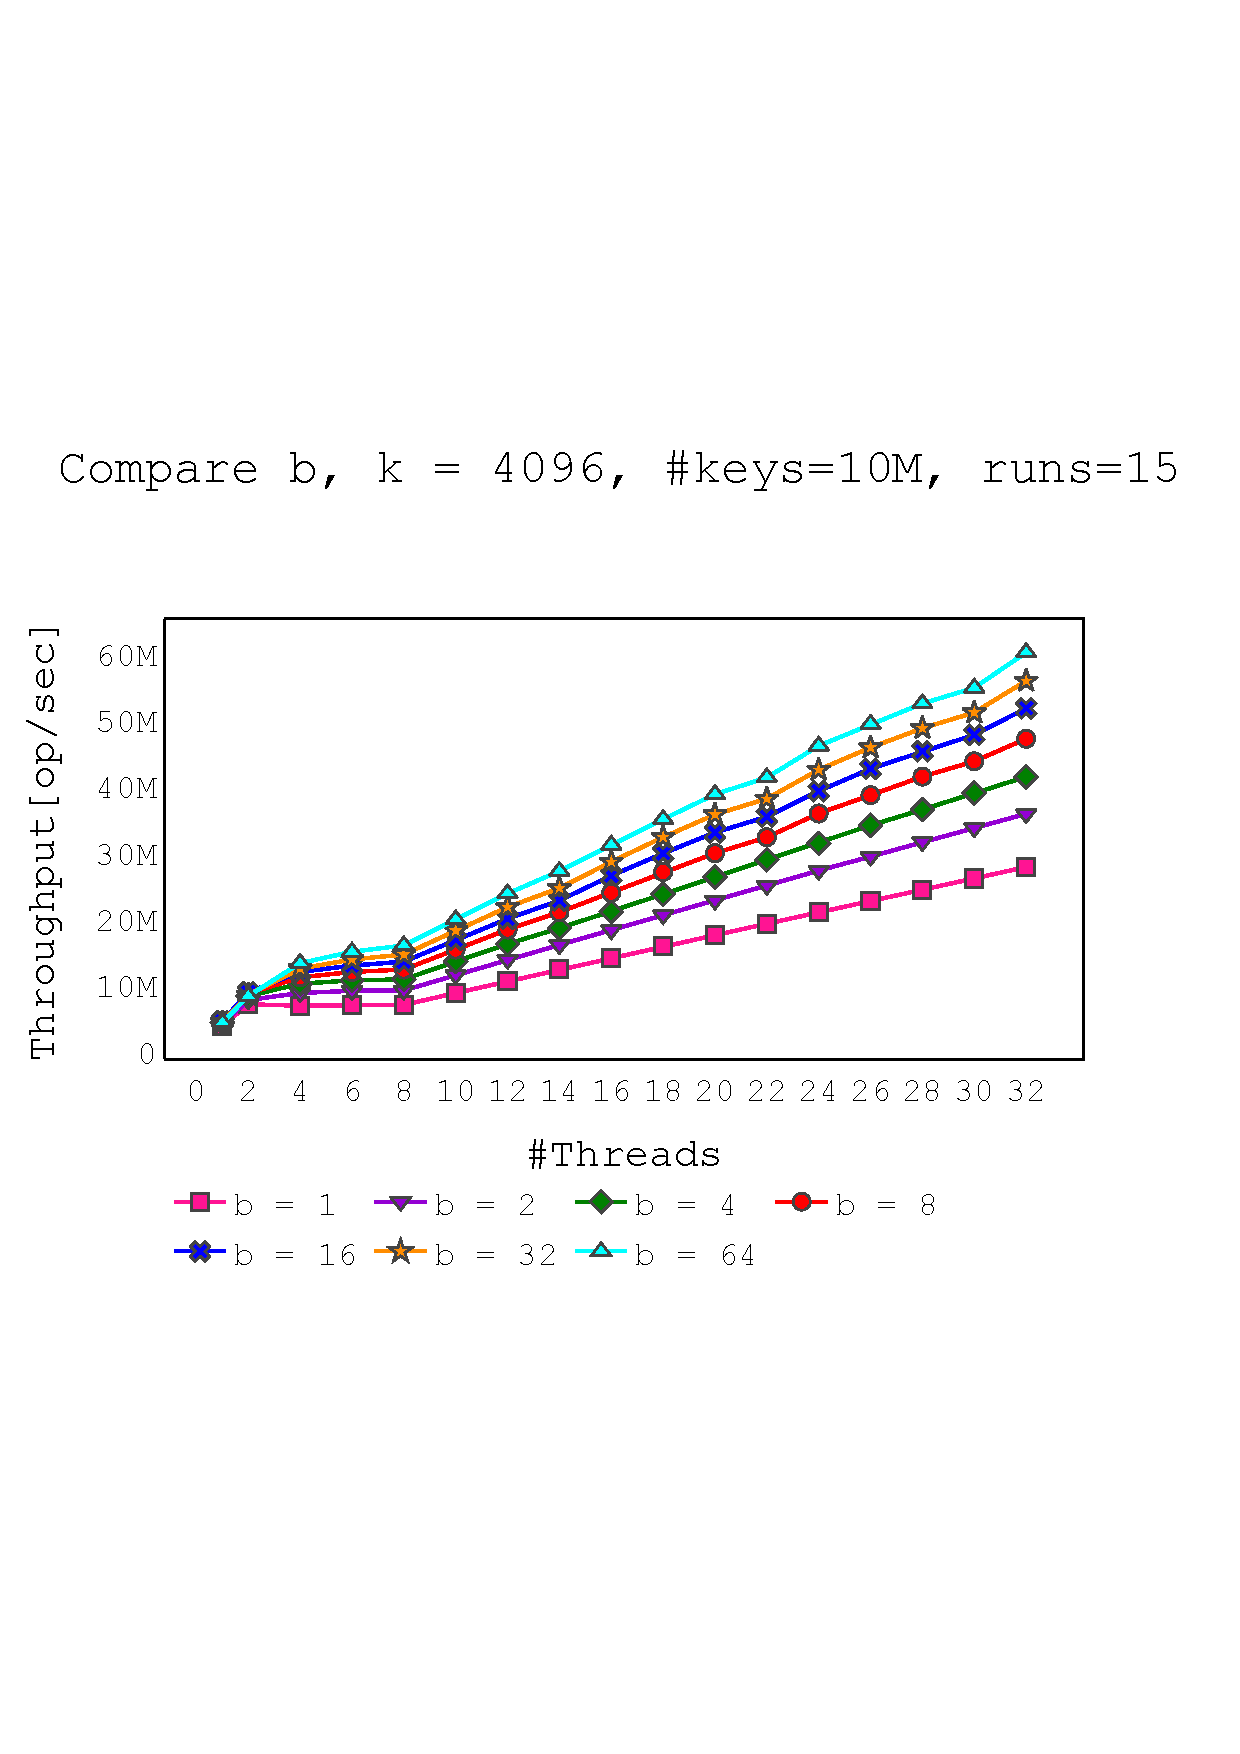
\includegraphics[width=0.7\textwidth,trim={0cm 7cm 1cm 10cm},clip]{graphics/graphs/parameters/oracle_Quancurrent_blocking_numa_compare_b_k4096_keys10M_Tup32_runs15_11-08-2022_20-12-56_flat.pdf}
    \caption{Update-only, \#keys = $10M$, $k=4096$.}
    \label{fig: throughput_update_compare_b}
    \end{subfigure}
\vfill
    \begin{subfigure}{\textwidth}
    \centering
    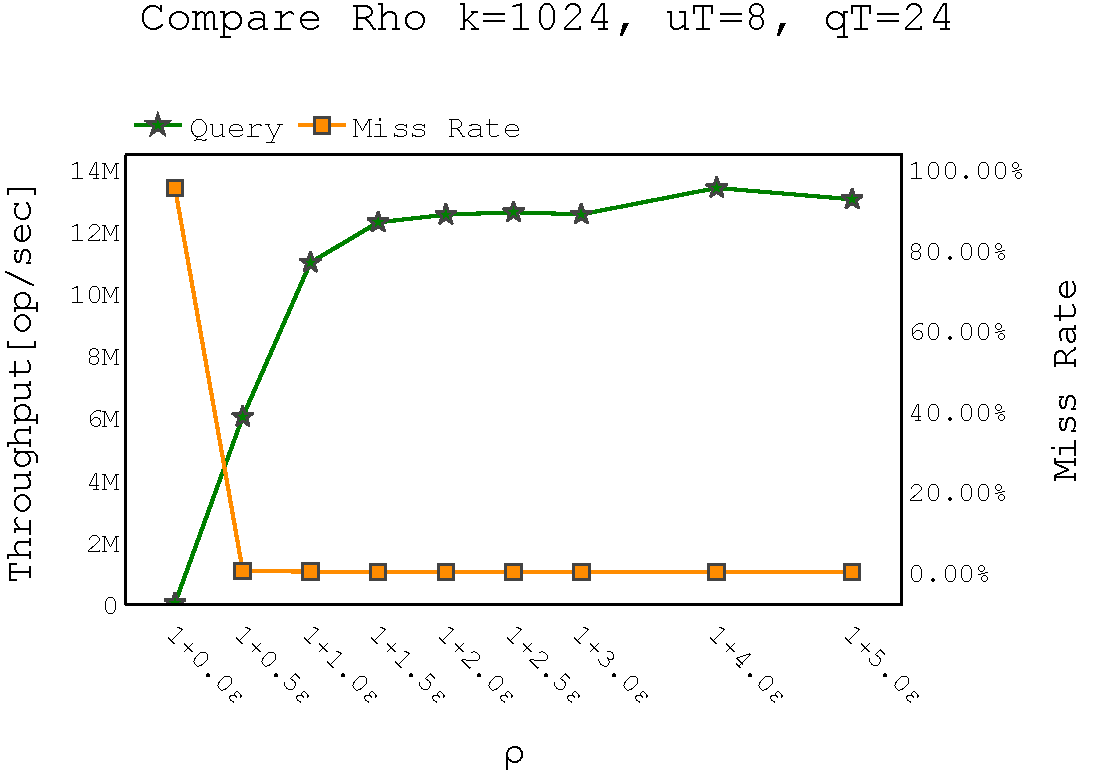
\includegraphics[width=0.7\textwidth,trim={0 0cm 0cm 0.7cm},clip]
    {graphics/graphs/parameters/oracle_Quancurrent_compare_rho_blocking_numa_k1024_b16_runs15_pre10M_pT1_keys10M_uT8_qT24_noUpdate_16-08-2022_09-20-38.pdf}
    \caption{$8$ update threads, $24$ query threads, \#keys = $10M$, $k=1024$ and $b=16$.}
    \label{fig: update_query_compare_rho}
    \end{subfigure}
\caption{\mysketch's parameters impact.}
\label{fig: parameters_exploration}
\end{figure*}

%============================================================
\section{Accuracy}
\label{sec:accuracy} 
%============================================================
To measure the estimate accuracy, we consider a query invoked in a quiescent state where no updates occur concurrently with the query. Figure~\ref{fig: accuracy_stderr} shows the standard error of 1M estimations in a quiescent state.%(with no concurrent updates). If the stream distribution does not change over time, this reflects the steady state estimation. While in theory, in order for \mysketch with $b=16$ and $N>1$ threads to provide the same error guarantee as the sequential Quantiles sketch with $k_{seq}$, we need to instantiate the sketch with the $k$ parameter larger by an order of magnitude. Figure~\ref{fig: accuracy_stderr} shows that in practice, in a quiescent state, \mysketch's estimations are similar to the sequential ones using the same $k$. 
We see that \mysketch's estimations are similar to the sequential ones using the same $k$, and improves with larger values of $k$ as known from the literature on sequential sketches~\cite{mergeables_summaries}.
\begin{figure}[h!]
    \centering
    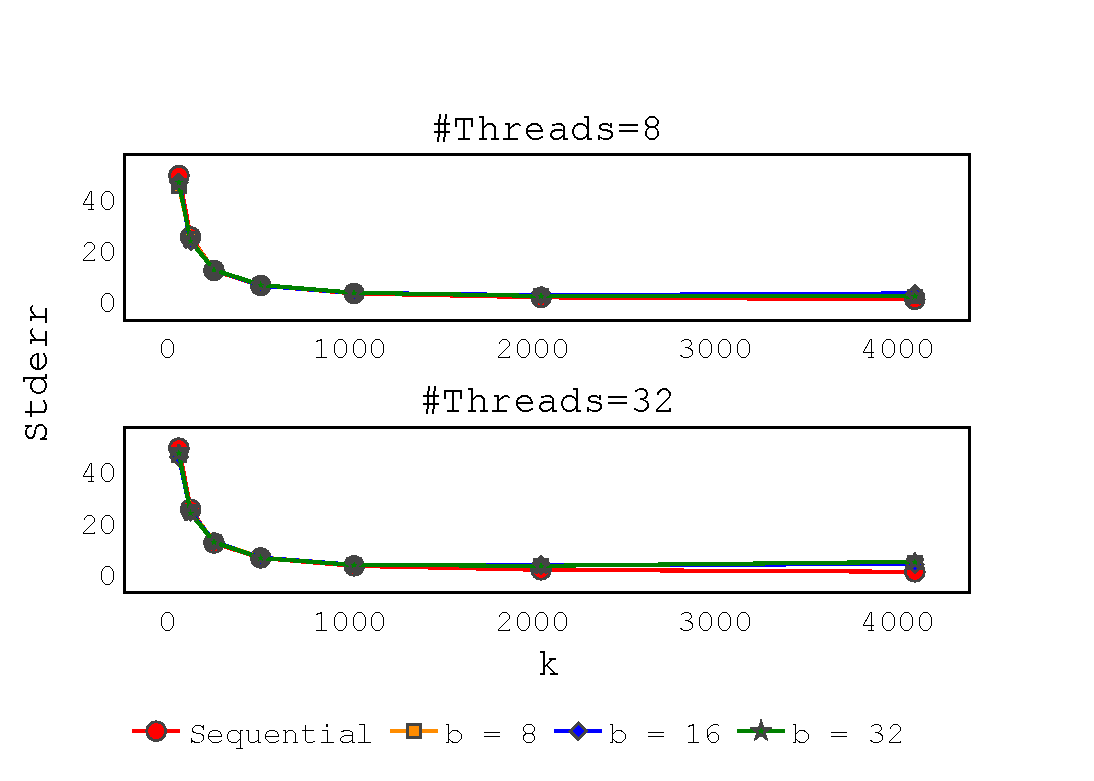
\includegraphics[width=0.8\textwidth,trim={0 0cm 0cm 1.7cm},clip]
    {graphics/graphs/accuracy/oracle_Quancurrent_block_numa_query_hist_stderr_qs_keys983040_runs1000_k_64_128_256_512_1024_2048_4096_b_8_16_32_T_8_32_11-08-2022_20-26-21.pdf}
    \caption{Standard error of estimation in quiescent state, keys = $1M$, runs = $1000$.}
    \label{fig: accuracy_stderr}
\end{figure}

To illustrate the impact of $k$ visually, Figure~\ref{fig:cdf} compares the distribution measured by \mysketch (red open-circles) to the exact (full information) stream distribution (green CDF filled-circles). In Figure~\ref{fig:intro-query-accuracy} (in the introduction), we depict the accuracy of \mysketch's estimate of a normal distribution with $k=1024$. Figure~\ref{fig:cdf_normal} (left) shows that when we reduce $k$ to $32$, the approximation is less tight while for $k=256$ (Figure~\ref{fig:cdf_normal} right) it is very accurate. We observe similar results for the uniform distribution in Figure~\ref{fig:cdf_uniform}. 
% We experimented with additional distributions with similar results, which are omitted due to space limitations. \todo[color=red]{ask if to remove}

\begin{figure}[h!]
\centering
    \begin{subfigure}[]{\textwidth}
        \centering
        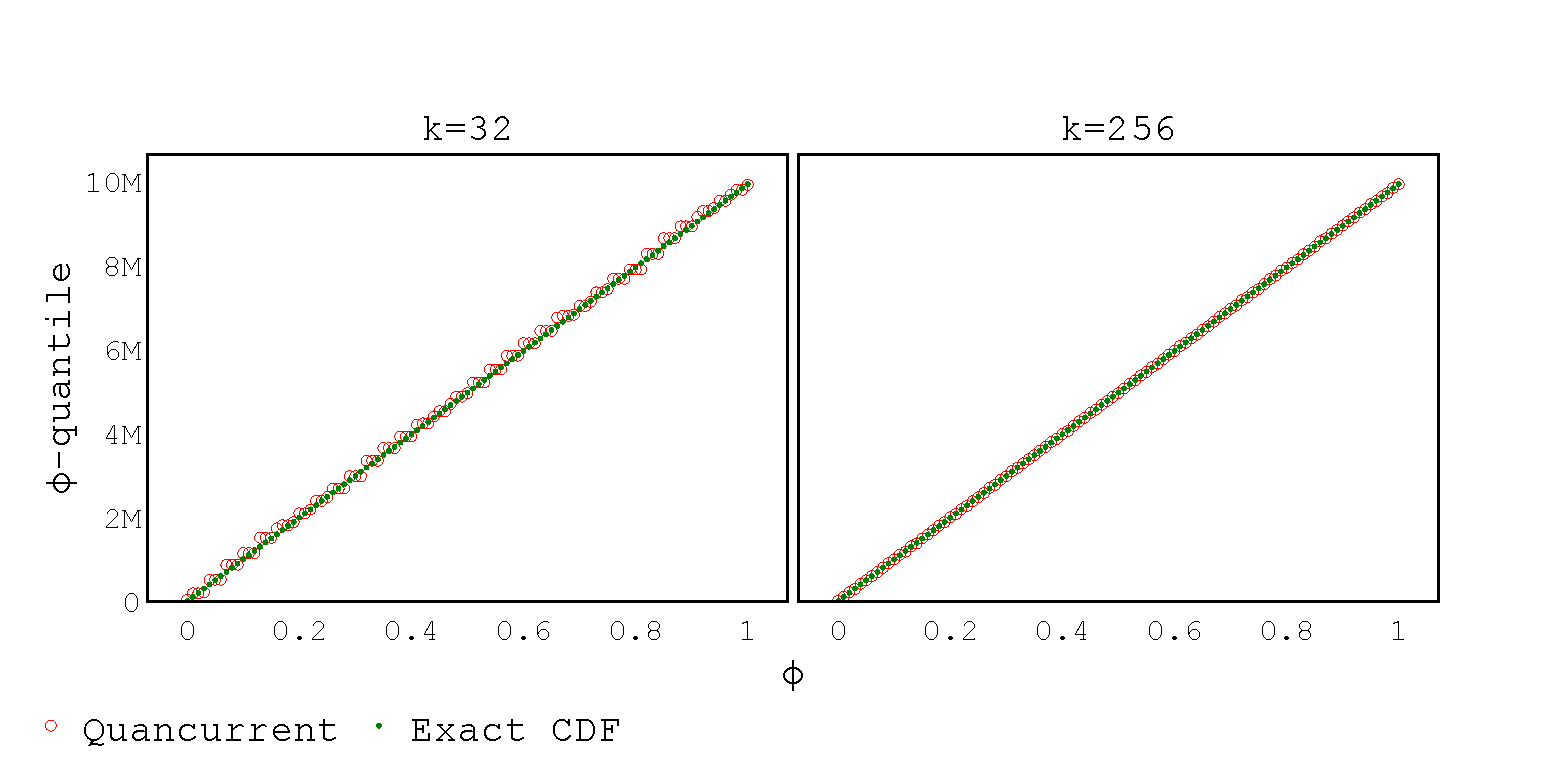
\includegraphics[width=0.8\textwidth,trim={0.1cm 0.2cm 1.5cm 1cm},clip]
        {graphics/graphs/accuracy/Oracle_Quancurrent_blocking_numa_cdf_uniform_ks_32_256_b16_keys10M_runs1_uT_32_qT1_snapshot1_17-09-2022_06-51-43.pdf}
        \caption{Uniform distribution.} \label{fig:cdf_uniform}
    \end{subfigure}
    
    \begin{subfigure}[]{\textwidth}
        \centering
        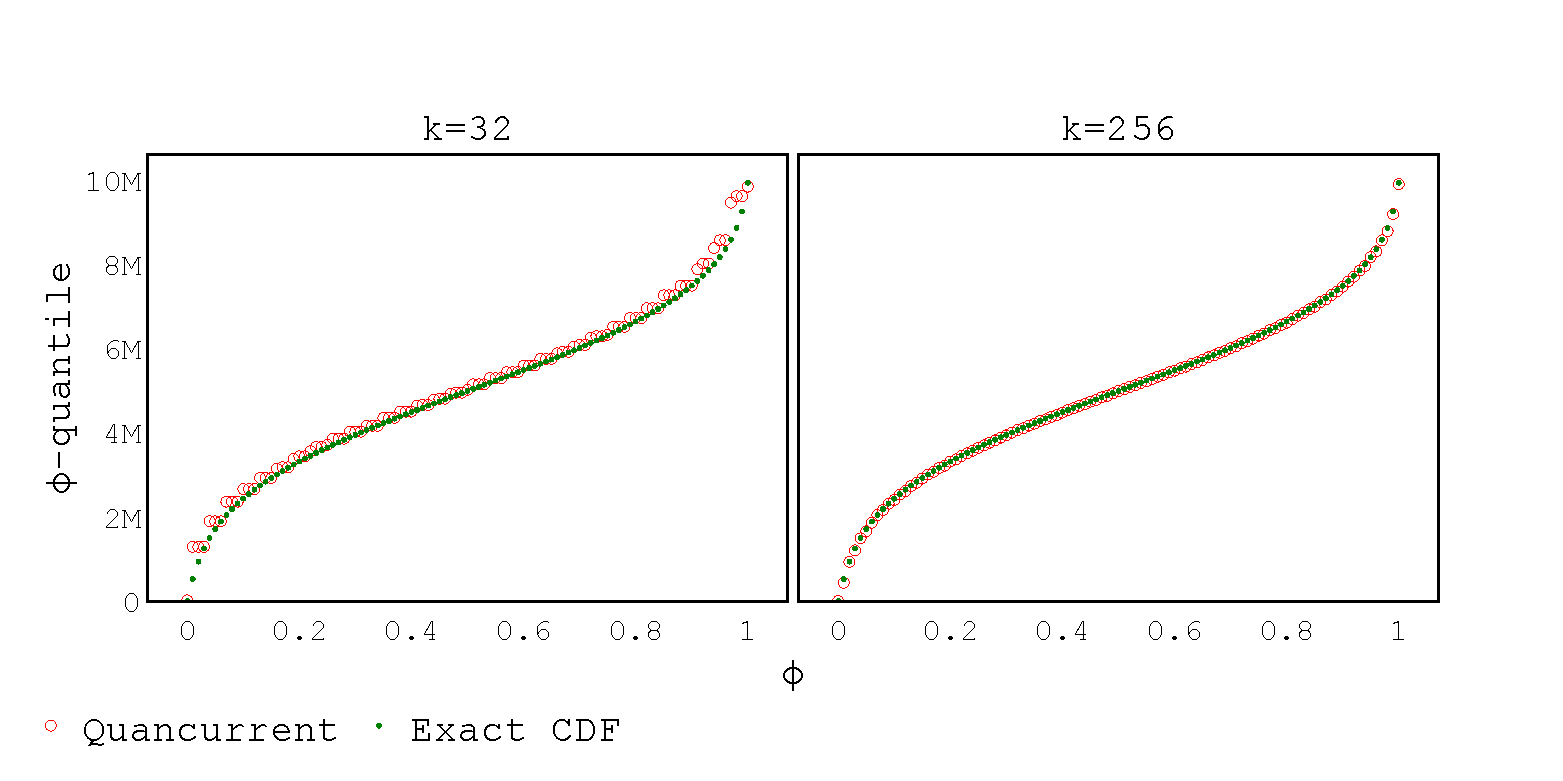
\includegraphics[width=0.8\textwidth,trim={0.1cm 0.2cm 1.5cm 1cm},clip]
        {graphics/graphs/accuracy/Oracle_Quancurrent_blocking_numa_cdf_normal_ks_32_256_b16_keys10M_runs1_uT_32_qT1_snapshot1_17-09-2022_06-51-43.pdf}
        \caption{Normal distribution.} \label{fig:cdf_normal}
    \end{subfigure}

\caption{\mysketch's $\phi$-quantiles vs. exact quantiles, with $32$ threads, $b=16$, and a stream size of $10M$.} \label{fig:cdf}
\end{figure}

%============================================================
\section{Comparison to state of the art}
\label{sec:compare} 
%============================================================
Finally, we compare \mysketch against a concurrent Quantiles sketch implemented within the FCDS framework~\cite{Rinberg_2020_fast_sketches}, the only previously suggested concurrent sketch we know that supports quantiles. Figure~\ref{fig:compare_FCDS_k4096} shows the throughput results (log scale) for $8$, $16$, $24$ and $32$ threads and $k=4096$.
FCDS satisfies relaxed consistency with a relaxation of up to $2NB$, where $N$ is the number of worker threads and $B$ is the buffer size of each worker. Recall that \mysketch's relaxation is at most $r = 4kS+(N-S)b$. For a fair comparison, we compare the two algorithms in settings with the same relaxation.

For $8$ update threads ($S=1$) and $b=2048$, the relaxation of \mysketch is $r\approx 30K$. The same relaxation in FCDS with the same number of update threads is achieved with a buffer size of $B=1920$.
With $8$ threads, \mysketch reaches a throughput of $22M\ ops/sec$ for a relaxation of $30K$ whereas FCDS reaches a throughput of $25M\ ops/sec$ for a much larger relaxation of $137K$. Also, with $32$ threads, \mysketch reaches a throughput of $62M\ ops/sec$ for a relaxation of $122K$, but FCDS only reaches a throughput of $19M\ ops/sec$ with a relaxation of more than $500K$.

Overall, we see that FCDS requires large buffers (resulting in a high relaxation and low query freshness) in order to scale with the number of threads. This is because, unlike \mysketch, FCDS uses a single thread to propagate data from all other threads' local buffers into the shared sketch. The propagation involves a heavy merge-sort, so large local buffers are required in order to offset it and keep the working threads busy during the propagation. In contrast, \mysketch's propagation is collaborative, with merge-sorts occurring concurrently both at the NUMA node level (in Gather\&Sort buffers) and at multiple levels of the shared sketch.
\todo[color=red]{consider put b,B values}
% \mysketch scales better for small relaxation then FCDS. This is because FCDS uses a single propagator thread and no shared buffers, and therefore requires much larger local buffers in order to offset the amount of work done by the propagator thread.



% \begin{figure}[]
%  \centering
%  \begin{minipage}[H]{0.45\textwidth}
%         \centering
%         \captionsetup{skip=0pt}
%         \captionof{table}{\mysketch vs. FCDS, k = 256, \#keys = 10M.}
%         % \resizebox{\textwidth}{} {
%         % \begin{tabular} {c{20pt}|l{30pt}|l{50pt}|c{25pt}c{25pt}|r{30pt}|r{50pt}}
%         \resizebox{\textwidth}{!}{%
%         \tiny
%         \begin{tabular} {@{}c|lc|cc|lc@{}} \toprule
%         %  & \multicolumn{6}{c}{k = 256} \\
%         % \cmidrule(r){2-7}
%          \multicolumn{1}{c}{}  & \multicolumn{3}{c|}{Quancurrent}  & \multicolumn{3}{c}{FCDS} \\  
%                 \cmidrule(r){1-7}
%         N      &    b    &   Throughput$[\frac{\textit{op}}{\textit{sec}}]$  &   \multicolumn{2}{c|}{r}  &   B       &   Throughput$[\frac{\textit{op}}{\textit{sec}}]$ \\ \midrule
%                 &       &                       &    \phantom{xxx}  &    \phantom{xxx}       &           &          \\[-\normalbaselineskip] % fake/empty row
%         8      &   1    &  \prefix{8.41E+06}    &   \multicolumn{2}{c|}{\prefix{1.02E+03}}   &    64     &    \prefix{5.60E+06}\\
%               &   4    &  \prefix{1.35E+07}    &   \multicolumn{2}{c|}{\prefix{1.06E+03}}   &    66     &    \prefix{5.60E+06}\\
%               &   8    &  \prefix{1.58E+07}    &   \multicolumn{2}{c|}{\prefix{1.09E+03}}   &    68     &    \prefix{5.70E+06}\\
%               &   16   &  \prefix{1.76E+07}    &   \multicolumn{2}{c|}{\prefix{1.14E+03}}   &    71     &    \prefix{5.70E+06}\\
%               &   32   &  \prefix{1.93E+07}    &   \multicolumn{2}{c|}{\prefix{1.25E+03}}   &    78     &    \prefix{5.70E+06}\\
%               &   64   &  \prefix{2.02E+07}    &   \multicolumn{2}{c|}{\prefix{1.47E+03}}   &    92     &    \prefix{5.80E+06}\\
%               &   128  &  \prefix{2.10E+07}    &   \multicolumn{2}{c|}{\prefix{1.92E+03}}   &    120    &    \prefix{5.90E+06}\\
%               &   256  &  \prefix{1.53E+07}    &   \multicolumn{2}{c|}{\prefix{2.82E+03}}   &    176    &    \prefix{6.00E+06}\\
%               &   512  &  \prefix{8.13E+06}    &   \multicolumn{2}{c|}{\prefix{4.61E+03}}   &    288    &    \prefix{6.10E+06}\\
%               &        &                       &   \multicolumn{2}{c|}{\prefix{8.19E+03}}   &    512    &    \prefix{3.01E+07}\\
%               &        &                       &   \multicolumn{2}{c|}{\prefix{1.54E+04}}   &    960    &    \prefix{1.25E+07}\\
%               &        &                       &   \multicolumn{2}{c|}{\prefix{2.97E+04}}   &    1856   &    \prefix{2.95E+07}\\
%         32     &   1    &  \prefix{6.44E+06}    &   \multicolumn{2}{c|}{\prefix{4.10E+03}}   &    64     &    \prefix{4.40E+06}\\
%               &   4    &  \prefix{6.28E+06}    &   \multicolumn{2}{c|}{\prefix{4.22E+03}}   &    66     &    \prefix{4.40E+06}\\
%               &   8    &  \prefix{6.31E+06}    &   \multicolumn{2}{c|}{\prefix{4.35E+03}}   &    68     &    \prefix{4.50E+06}\\
%               &   16   &  \prefix{6.27E+06}    &   \multicolumn{2}{c|}{\prefix{4.54E+03}}   &    71     &    \prefix{4.40E+06}\\
%               &   32   &  \prefix{6.13E+06}    &   \multicolumn{2}{c|}{\prefix{4.99E+03}}   &    78     &    \prefix{4.50E+06}\\
%               &   64   &  \prefix{5.80E+06}    &   \multicolumn{2}{c|}{\prefix{5.89E+03}}   &    92     &    \prefix{4.60E+06}\\
%               &   128  &  \prefix{5.90E+06}    &   \multicolumn{2}{c|}{\prefix{7.68E+03}}   &    120    &    \prefix{4.80E+06}\\
%               &   256  &  \prefix{6.38E+06}    &   \multicolumn{2}{c|}{\prefix{1.13E+04}}   &    176    &    \prefix{5.20E+06}\\
%               &   512  &  \prefix{6.12E+06}    &   \multicolumn{2}{c|}{\prefix{1.84E+04}}   &    288    &    \prefix{5.40E+06}\\
%               &        &                       &   \multicolumn{2}{c|}{\prefix{3.28E+04}}   &    512    &    \prefix{2.12E+07}\\
%               &        &                       &   \multicolumn{2}{c|}{\prefix{6.14E+04}}   &    960    &    \prefix{1.11E+07}\\
%               &        &                       &   \multicolumn{2}{c|}{\prefix{1.19E+05}}   &    1856   &    \prefix{1.93E+07}\\ 
%         \bottomrule
%         \end{tabular} 
%         }
%   \end{minipage}
%     \par\bigskip
%     \begin{minipage}[H]{0.45\textwidth}
%     % \centering
%     % \rule{5.5cm}{2.6cm} % Height changed from 3.6cm to 2.6cm
%     % \captionof{figure}{A table beside a figure}
%     \centering
%     \includegraphics[width=\textwidth,trim={0.1cm 0.2cm 1.9cm 0.1cm},clip]
%     {images/graphs/FCDS/oracle_Quancurrent_vs_FCDS_blocking_numa_update_k256_keys10M_T8_32_runs15_equal_relax_log_scale_largeB_26-06-2022_14-04-13.pdf}
%     \captionof{figure}{\mysketch vs. FCDS, k = 256.}
%     \label{fig: FCDS k256}
%   \end{minipage}
% \end{figure}

\begin{figure}[h]
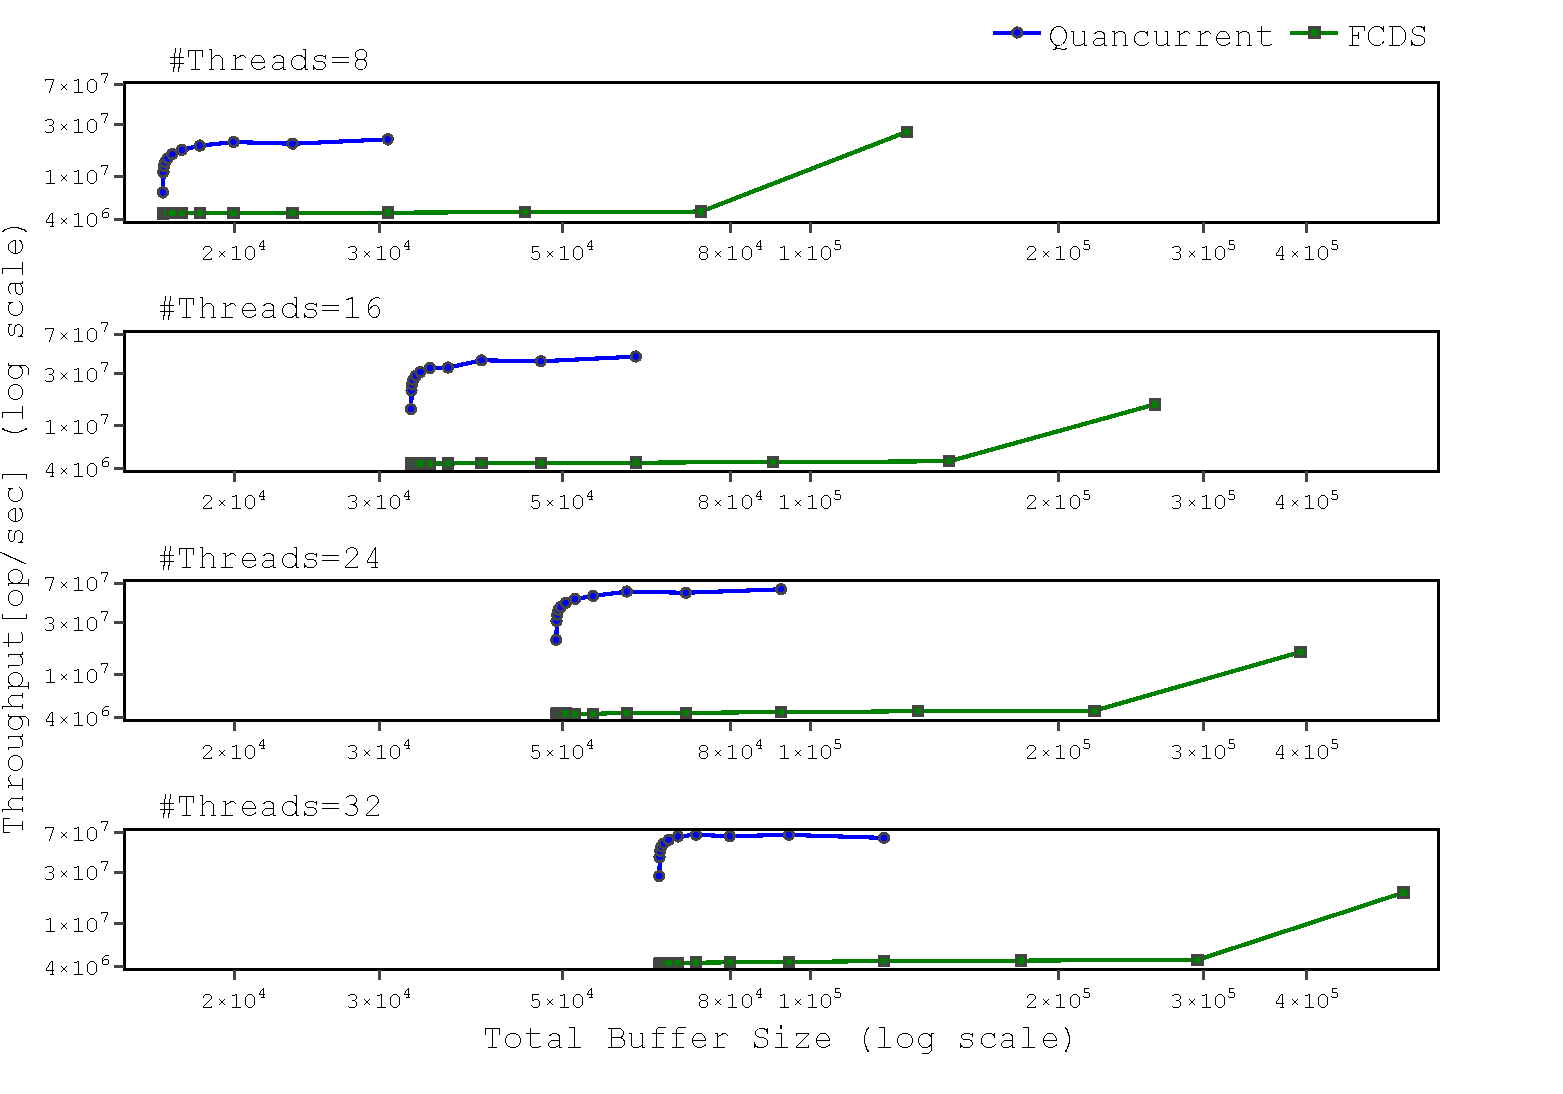
\includegraphics[width=\textwidth,trim={0cm 0cm 0cm 0cm},clip]
{graphics/graphs/FCDS/oracle_Quancurrent_vs_FCDS_block_numa_up_k4096_keys10M_T8-32_runs15_equal_relax_log_largeB_rm_last2_diff_axes_name_16-09-2022_18-59-50.pdf}
\caption{\mysketch vs. FCDS, $k=4096$.}
\label{fig:compare_FCDS_k4096}
\end{figure}
